\section{K1.8BR spectrometer system}
Figure \ref{fig:spectrometer} shows the K1.8BR spectrometer system which we have constructed in the K1.8BR experimental area. The spectrometer consists of a beam line spectrometer, a cylindrical detector system that surrounds the liquid $^3$He target system to detect the decay particles from the target region, a beam sweeping magnet, and a neutron and a proton time-of-flight counters located $\sim$15~m downstream from the target position. In the successive 4 sections, details of these components are described.
  \begin{figure}[]
   \begin{center}
    \includegraphics[width=\columnwidth]{ptep/fig/spectrometer.eps}
    \caption{Schematic view of the K1.8BR spectrometer.
%    The spectrometer consists of a beam line spectrometer, a
%    cylindrical detector system that surrounds the liquid
%    $^3$He/$^4$He/D$_2$ target system to detect the decay particles from
%    the target region, a beam sweeping magnet, and a neutron
%    time-of-flight counter located $\sim$15~m downstream from the target
%    position.
    }
    \label{fig:spectrometer}
   \end{center}
  \end{figure}  

\section{Detectors for kaon beam}
A schematic view of the beam analyzing part is shown in Fig.~\ref{fig:beamline}. It is composed of beam line magnets, trigger counters, beam trackers, and a kaon identification counter. The beam trigger is generated by a coincidence signal of a beam hodoscope detector (BHD) and a time zero counter (T0); the flight length between the BHD and T0 is $\sim$7.7~m. We additionally installed a beam definition counter (DEF) just upstream of the target to suppress the trigger rate.
The kaon beam with momentum around 1.0~GeV/$c$ is identified by using an aerogel Cherenkov counter (AC) with a refractive index of 1.05. The kaon beam is tracked with two beam trackers -- a beam line chamber 1 (BLC1) and a beam line chamber 2 (BLC2) -- and the momentum of the kaon is analyzed with this tracking information together with the beam optics of the D5 beam line magnet. Finally, beam trajectory just upstream of the experimental target is detected by a drift chamber (BPC) to determine the reaction vertex precisely.
  \begin{figure}[]
   \begin{center}
    \includegraphics[width=0.6\columnwidth]{ptep/fig/beamline.eps}
    \caption[Schematic view of the beam line spectrometer.]{Schematic view of the beam line spectrometer, which
    consists of trigger counters (BHD,T0 and DEF), beam line
    chambers (BLC1, BLC2 and BPC), and a kaon identification counter (AC).}
    \label{fig:beamline}
   \end{center}
  \end{figure}  

\subsection{Trigger counters}
\subsubsection{BHD and T0}
The BHD and T0 are segmented plastic scintillation counters
located downstream of the D3 and the D5 magnet, respectively.
The T0 signal is used as the event time-zero signal.

The BHD has an effective area of 400~mm (horizontal) $\times$ 160~mm
(vertical) segmented into 20 units horizontally, and T0 is 160~mm
(horizontal) $\times$ 160~mm (vertical) segmented into 5 units
horizontally.
To avoid over-concentration of the beam on one segment, T0 is
rotated by 45 degrees in the $xy$ plane.
The BHD scintillator is made of Saint-Gobain BC412 with a unit size of
160~mm (height) $\times$ 20~mm (width) $\times$ 5~mm (thickness).
The unit size of T0 made of the Saint-Gobain BC420 scintillator is 160 mm
(height) $\times$ 32~mm (width) $\times$ 10~mm (thickness).
In both of the trigger counters, the scintillation light is transferred
to a pair of 3/4~inch Hamamatsu H6612B photomultipliers that are
attached to the top and bottom ends.
Since the coincidence rate of the top and bottom photomultipliers is expected to
reach $\sim$1~M counts per spill, the high voltage boosters of all the
photomultipliers are modified to supply adequate current to the last three
dynodes.
Discriminated signals from the top and bottom photomultipliers
are coincidenced and provide the timing of each segment.
%The typical TOF resolution between the BHD and T0 is 160~ps ($\sigma$) after a slewing correction is applied.

\subsubsection{Beam definition counter}
The DEF is installed just upstream of the target vacuum vessel to improve data quality and an efficiency of data acquisition. Under the current magnetic spectrometer setup, only half of the kaon beam hits the liquid $^3$He target due to the large beam spot size. So the DEF is used for selecting the central region of the beam at the trigger level by adding the DEF signal to the beam trigger made by the coincidence signal of the BHD and T0.

The DEF is required to be a thin detector to reduce energy losses, a small detector within the BPC radial size, and operated in the magnetic field. To fulfill these requirements, a thin scintillation counter array is adopted. The scintillation light is collected by a wavelength-shifting (WLS) fiber, Kuraray Y-11(200)M with 1 mm diameter. The light from the fiber is read from both ends with multi-pixel photon counters (MPPCs) made by Hamamatsu (S10362-11-100C). The WLS fiber is embedded in a 3 mm thick scintillator (ELJEN EJ-202) with 1.1mm depth, and fixed by optical cement ELJEN EJ-510 as illustrated in Fig. \ref{fig-DEF}. 
MPPCs are coupled to the fiber by using GOMI connectors developed by the T2K experiment\cite{Kawamuko:2006zz}. 
Because of $\sim$ 6 ns decay time of the WLS fiber, the time resolution is expected to be not as good as 1 ns.  

The trigger rate was successfully suppressed by $\sim$30\% after the installation of the DEF.   

\begin{figure}[]
\begin{center}
\includegraphics[width=\columnwidth]{./illustrator/DEF.eps}
\caption{Schematic drawing of the DEF counter.}
\label{fig-DEF}
\end{center}
\end{figure}  

\subsection{Kaon identification counter}
The AC located downstream of T0 is used to identify the kaon at the trigger level. Figure \ref{fig-ACthre} shows relations of the momentum and critical reflection index for pion and kaon. In our case, an aerogel radiator with a reflection index of 1.05 
%, produced by ..... .,
is used as a threshold-type Cherenkov counter to reject pions with momenta around 1.0 GeV/$c$. The AC, as show in Fig. \ref{fig-AC}, 
has an effective area of 180~mm (width) $\times$ 100~mm (height) $\times$ 100~mm (thickness) which covers the whole distribution of the kaon beam. Cherenkov photons radiated in the beam direction are diffused in the aerogel and reflected by the thin mirror foils around it, and part of them reached at four photomultipliers on the top and bottom. Three-inch fine-mesh type photomultipliers (Hamamatsu R5543) are used to compete with fringing fields of the D5 magnet and the CDS magnet. 
AC pulse height distributions for 1.0 GeV/$c$ pions and kaons, which are obtained by summing ADC spectra of the four photomultipliers, are shown in Fig.~\ref{fig:AC_ADC}. In the figures, particle identifications are achieved by the TOF method between the BHD and T0 in off-line analysis. 
On-line pion identification is performed by the AC at a threshold level of $\sim$7 photoelectrons. A pion detection efficiency of $>$99\% is achieved, whereas the miss identification ratio of a kaon as a pion is $\sim$1\%.

\begin{figure}[]
\begin{center}
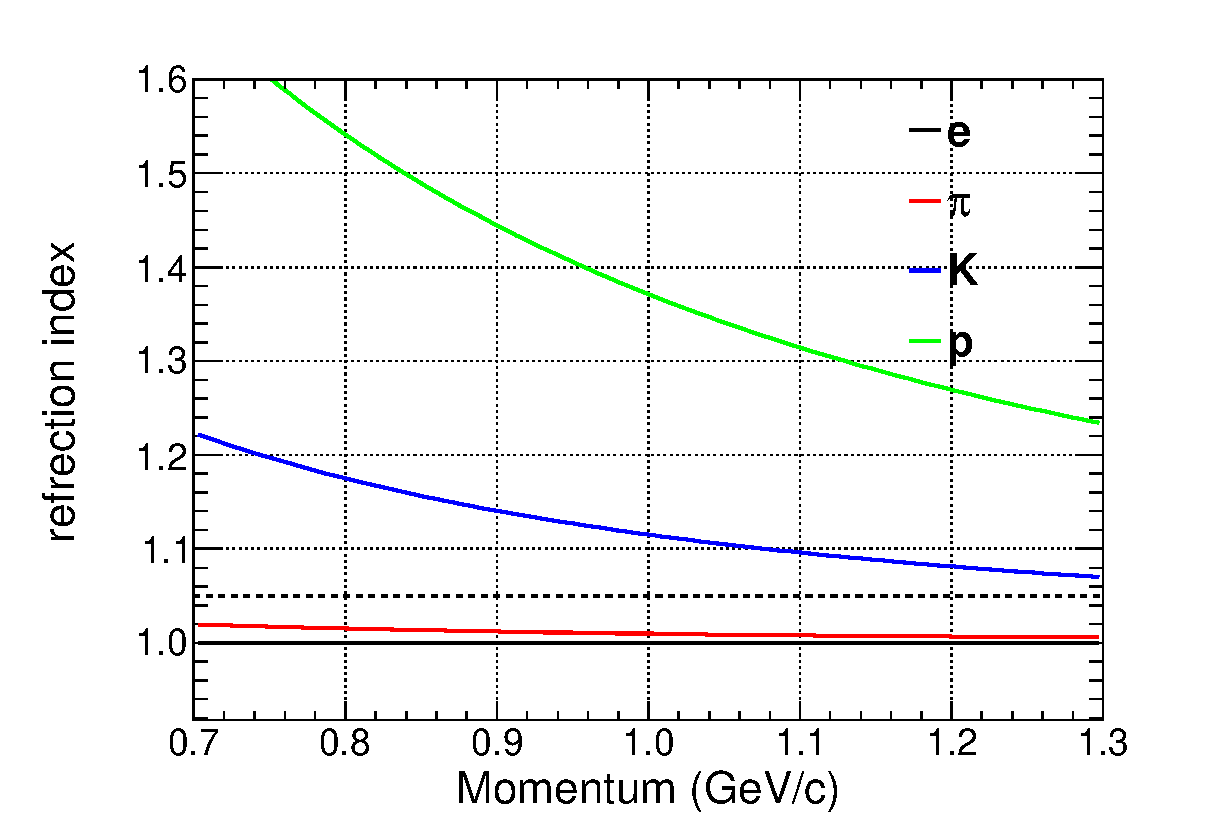
\includegraphics[width=10cm]{./fig/ACthre.eps}
\caption[Threshold of reflection index for Cherenkov radiation as a function of the momentum.]{Threshold of reflection index for Cherenkov radiation as a function of the momentum. The horizontal dotted line shows the reflection index of the Aerogel (n=1.05).}
\label{fig-ACthre}
\end{center}
\end{figure}  

\begin{figure}[]
\begin{center}
\includegraphics[width=\columnwidth]{./illustrator/newac.eps}
\caption{Schematic drawing of the aerogel Cherenkov counter.}
\label{fig-AC}
\end{center}
\end{figure}  

\begin{figure}[]
\begin{center}
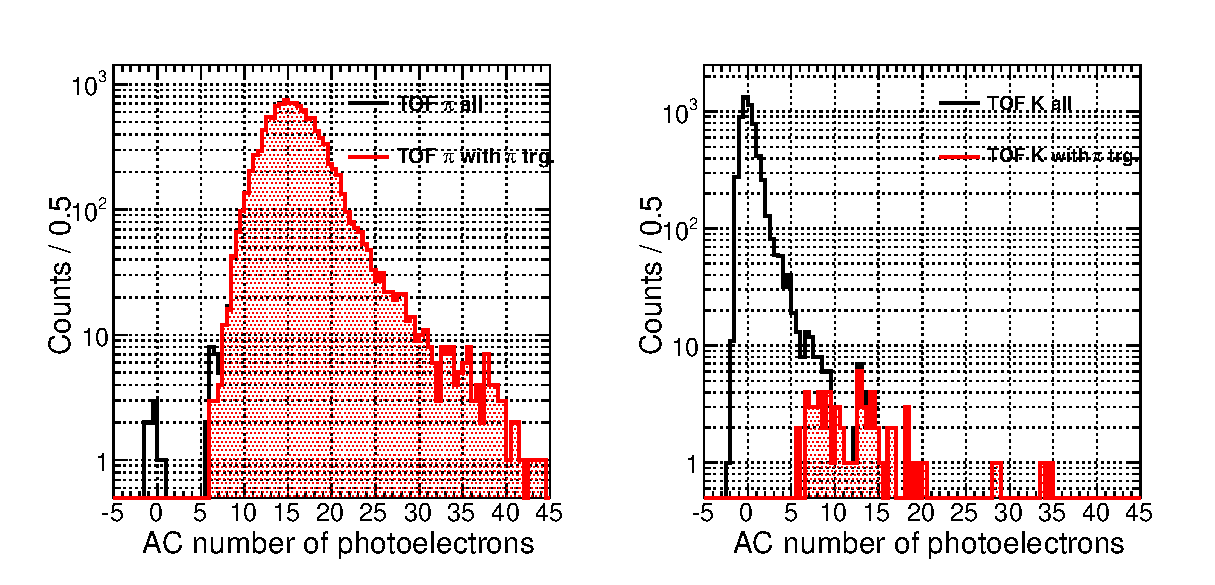
\includegraphics[width=\columnwidth]{./fig/beam-ac2.eps}
 \caption[AC Pulse height distributions for 1.0 GeV/$c$ pions and kaons.]{AC Pulse height distributions for 1.0 GeV/$c$ (left) pions and
 (right) kaons.
 Black histograms represent (left) pions and (right) kaons identified
 with the TOF between the BHD and T0.
 Filled histograms represent the events identified as pions by the AC. 
 }
 \label{fig:AC_ADC}
\end{center}
\end{figure}

\subsection{Beam momentum analyzer}
Two similar planar drift chambers, BLC1 and BLC2, are installed in the entrance and the exit of the D5 magnet. Their tracks are connected by a second-order transport matrix to reconstruct the kaon beam momentum. Assuming 200 $\mu$m spatial resolutions for BLC1 and BLC2, the momentum resolution of the spectrometer is estimated to be 1 $\times 10^{-3}$, which is good enough for our experiment.% as discussed in \ref{sec-require}. 
The magnetic field of D5 is monitored during the experiment with a high-precision Hall probe, Lakeshore 475 ( $\sim10^{-5}$ T resolution). The fluctuation of the magnetic field was $\sim 2\times10^{-4}$ corresponding to 0.2 MeV/$c$ for the 1 GeV/$c$ beam. We also install a helium bag into the D5 magnet to suppress the scattering effects in the air.  
\subsubsection{BLC1 and BLC2}
BLC1 consists of two sets of drift chamber with the same design, BLC1a and BLC1b, which have 8 layers with a $UU'VV'UU'VV'$ configuration. In the $U$ and $V$ layers the wires are tilted by $\pm$ 45 degrees. Each layer contains 32 sense wires with a drift length of 4~mm corresponding to an effective area of 256~mm $\times$ 256~mm. The number of readout channels is 256 for both BLC1a and BLC1b, which are installed 300~mm apart upstream of the D5 magnet.

BLC2 is similar to BLC1; BLC2 consists of two sets of the same drift chamber, BLC2a and BLC2b. Each chamber has a $UU'VV'UU'VV'$ configuration and 32 sense wires per layer, i.e, the number of readout channels is 256 for both BLC2a and BLC2b. In the $U$ and $V$ layers the wires are tilted by $\pm$ 45 degrees. The drift length of 2.5~mm corresponds to an effective area of 160~mm $\times$ 160~mm. BLC2a and BLC2b are installed 275~mm apart downstream of the D5 magnet.

Both BLC1 and BLC2 use 12.5 $\mu$m diameter gold-plated tungsten wires with 3\% rhenium and 75 $\mu$m diameter copper-beryllium wires for the sense and potential wires, respectively. The cathode planes are made of 12.5 $\mu$m aluminized Kapton.
The readout electronics of both chambers consist of a preamplifier card with amplifier-shaper-discriminator ICs (ASD, SONY-CXA3653Q, %~\cite{ASD}, 
$\tau$ = 16~ns) mounted on the chambers, an LVDS-ECL converter, and a TDC.
The output signal of the ASD board is sent to the LVDS-ECL converter board via 7~m long twisted-pair cables. From the LVDS-ECL converter, the signal is transferred to the counting house with 50~m long twisted-pair cables.
The chamber gas is an argon-isobutane mixture passed through a methylal (dimethoxy-methane) bubbler at a refrigerator temperature of 4 $^\circ\mathrm{C}$ with a ratio of 76\% (Ar), 20\% (isobutane) and 4\% (methylal).
The operating voltages of BLC1 and BLC2 are set at -1.35~kV on both the potential wires and the cathode planes.

\subsection{Vertex chamber}
A backward proton chamber (BPC) is originally developed to detect backward-scattered particles in another experiment, spectroscopic study of $\Lambda$(1405) (J-PARC E31). However, it also works as a kaon beam tracker to determine the reaction vertex point precisely.  

The BPC is a compact circular planar drift chamber located just before the target system whose size is 168~mm in diameter and 89.7~mm in height. Figure~\ref{fig:BPC} shows the design of the BPC, which consists of 8 layers with an $XX'YY'X'XY'Y$ configuration, where the wires of the $Y$ layer are tilted by 90 degrees. Each layer contains 15 sense wires with a drift length of 3.6~mm corresponding to an effective area with a 111.6~mm diameter. The number of readout channels is 120.
The cathode planes are made of 9~$\mu$m carbon aramid foil, and the sense and potential wires, readout electronics, and gas mixture of the BPC are the same as those for the beam line chambers. The operational voltage of the BPC is set at -1.45~kV on both the potential wires and the cathode planes. 
\\

Figure \ref{fig-bldccell} shows the cell geometries of the beam-drift chambers. The parameters of the beam line chambers are summarized in Table \ref{tab-chamber}.% including FDC1, whose details will be described in Sec. \ref{sec-fdc}. 

  \begin{figure}[]
   \begin{center}
    \includegraphics[width=0.8\columnwidth]{ptep/fig/BPC.eps}
    \caption[Design of the BPC]{Design of the BPC (all dimensions in mm).}
    \label{fig:BPC}
   \end{center}
  \end{figure}

  \begin{figure}[]
   \begin{center}
    \includegraphics[width=0.8\columnwidth]{illustrator/chambercell.eps}
    \caption[Cell geometries of beam-line drift chambers.]{Cell geometries of (a)BLC1/2, (b)BPC, and (c)FDC1.}
    \label{fig-bldccell}
   \end{center}
  \end{figure}

\begin{landscape}
\begin{table}[]
\caption{Summary of the beam-line chamber parameters.}
\begin{center}
\begin{tabular}{l|cccc|c|c} 
\hline\hline													
	&	BLC1a	&	BLC1b	&	BLC2a	&	BLC2b	&	BPC	&	FDC1	\\
\hline													
number of planes	&	8	&	8	&	8	&	8	&	8	&	6	\\
plane configuration	&	\footnotesize{UU'VV'UU'VV'}	&	\footnotesize{UU'VV'UU'VV'}	&	\footnotesize{UU'VV'UU'VV'}	&	\footnotesize{VV'UU'VV'UU'}	&	\footnotesize{XX'YY'X'XY'Y}	&	\footnotesize{UU'XX'VV'}	\\
\shortstack{number of sense wires \\ in a plane}	&	32	&	32	&	32	&	32	&	15	&	64	\\
wire spacing (mm)	&	4	&	4	&	2.5	&	2.5	&	3.6	&	3	\\
effective area (mm)	&	256 $\times$ 256	&	256 $\times$ 256	&	160 $\times$ 160	&	160 $\times$ 160	&	111.6 mm$\phi$	&		\\
\hline													
Sense wire	&	\multicolumn{5}{c|}{}									&		\\
~~material	&	\multicolumn{5}{c|}{Au-plated W (3\% Re)}									&	Au-W(Re)	\\
~~diameter ($\mu m$)	&	\multicolumn{5}{c|}{ 12}									&	20	\\
\hline													
Potential wire	&	\multicolumn{5}{c|}{}									&	(field wire)	\\
~~material 	&	\multicolumn{5}{c|}{Au-plated Cu-Be}									&	Au-Al	\\
~~diameter ($\mu m$)	&	\multicolumn{5}{c|}{ 75}									&	80	\\
\hline													
Cathode plane	&	\multicolumn{4}{c|}{}							&		&	(shield wire)	\\
~~material	&	\multicolumn{4}{c|}{alminized-Kapton}							&	Cu aramid	&	Au-Al	\\
~~thickness ($\mu m$)	&	\multicolumn{4}{c|}{12.5}	&	9	&	80	\\
\hline													
Gas	&	\multicolumn{6}{c}{ Ar : isoC$_4$H$_{10}$ : Metylal = 76 : 20 :4}											\\
flow (cc/min)	&	\multicolumn{6}{c}{100}											\\
%plane efficiency 	&	$>$ 99\%	&	$>$ 99\%	&	$>$ 99\%	&	$>$ 99\%	&	$>$ 99\%	&	$>$ 99\%	\\
\hline													
operation voltage	&		&		&		&		&		&		\\
potential 	&	-1.35	&	-1.35	&	-1.35	&	-1.35	&	-1.5	&	-1.8	(field)\\
cathord	&	-1.35	&	-1.35	&	-1.35	&	-1.35	&	-1.5	&	-1.8	(shield)\\
%guard	&	-	&	-	&	-	&	-	&	-	&	-1.85	\\
\hline\hline										
\end{tabular}
\end{center}
\label{tab-chamber}
\end{table}%
\end{landscape}
													
